\section{Experiments}


\label{sec:exp}
% In this section, we first introduce datasets and our novel evaluation protocol on ScanNet, which preserves not only the rendering quality but also provides a fair comparison on 3D point clouds via a novel semantic propagation method.
\subsection{Experimental setup}
\label{exp:setup}

\textbf{Datasets.}
We evaluate on the two reference datasets for this task: LERF-OVS~\cite{qin2024langsplat} and ScanNet-v2~\cite{dai2017scannet}. LERF-OVS is derived from the LERF dataset of Kerr \etal~\cite{kerr2023lerf}, where we evaluate open-vocabulary object selection in both 2D and 3D. 
For the 2D evaluation, we follow the protocol of LERF~\cite{kerr2023lerf}. For the 3D evaluation, we follow OpenGaussian~\cite{wu2024opengaussian}. On ScanNet, we evaluate 3D semantic segmentation. Previous evaluation protocols~\cite{wu2024opengaussian,li2024instancegaussian} freeze the growth of 3D Gaussians, which degrades photometric fidelity. In contrast, we allow full optimization of the 3D Gaussians, resulting in misalignment between the optimized Gaussians and the ground-truth point cloud. We therefore adapt the evaluation protocol in~\cite{drsplat25} by propagating pseudo ground-truth labels to the Gaussians. Details are provided in the Appendix~\ref{subsec:eval_prot}. 
% All results in each table follow the same protocol.

\textbf{Implementation Details.} 
We generate SAM~\cite{kirillov2023sam} masks at subpart, part, and whole object granularities. We use OpenCLIP ViT-B/16~\cite{radford2021clip} and the \texttt{gsplat} rasterizer~\cite{ye2025gsplat}. We apply direct feature aggregation in the 512-dimensional space following~\cite{cheng2024occam}, combined with our proposed training-free method. The entire process requires only 10 seconds to one minute per scene (depending on scene scale), thanks to our effective cross-view feature aggregation and streaming updates at constant memory. For all experiments, we used an NVIDIA RTX 4090 GPU.

\begin{figure*}[t]
\centering
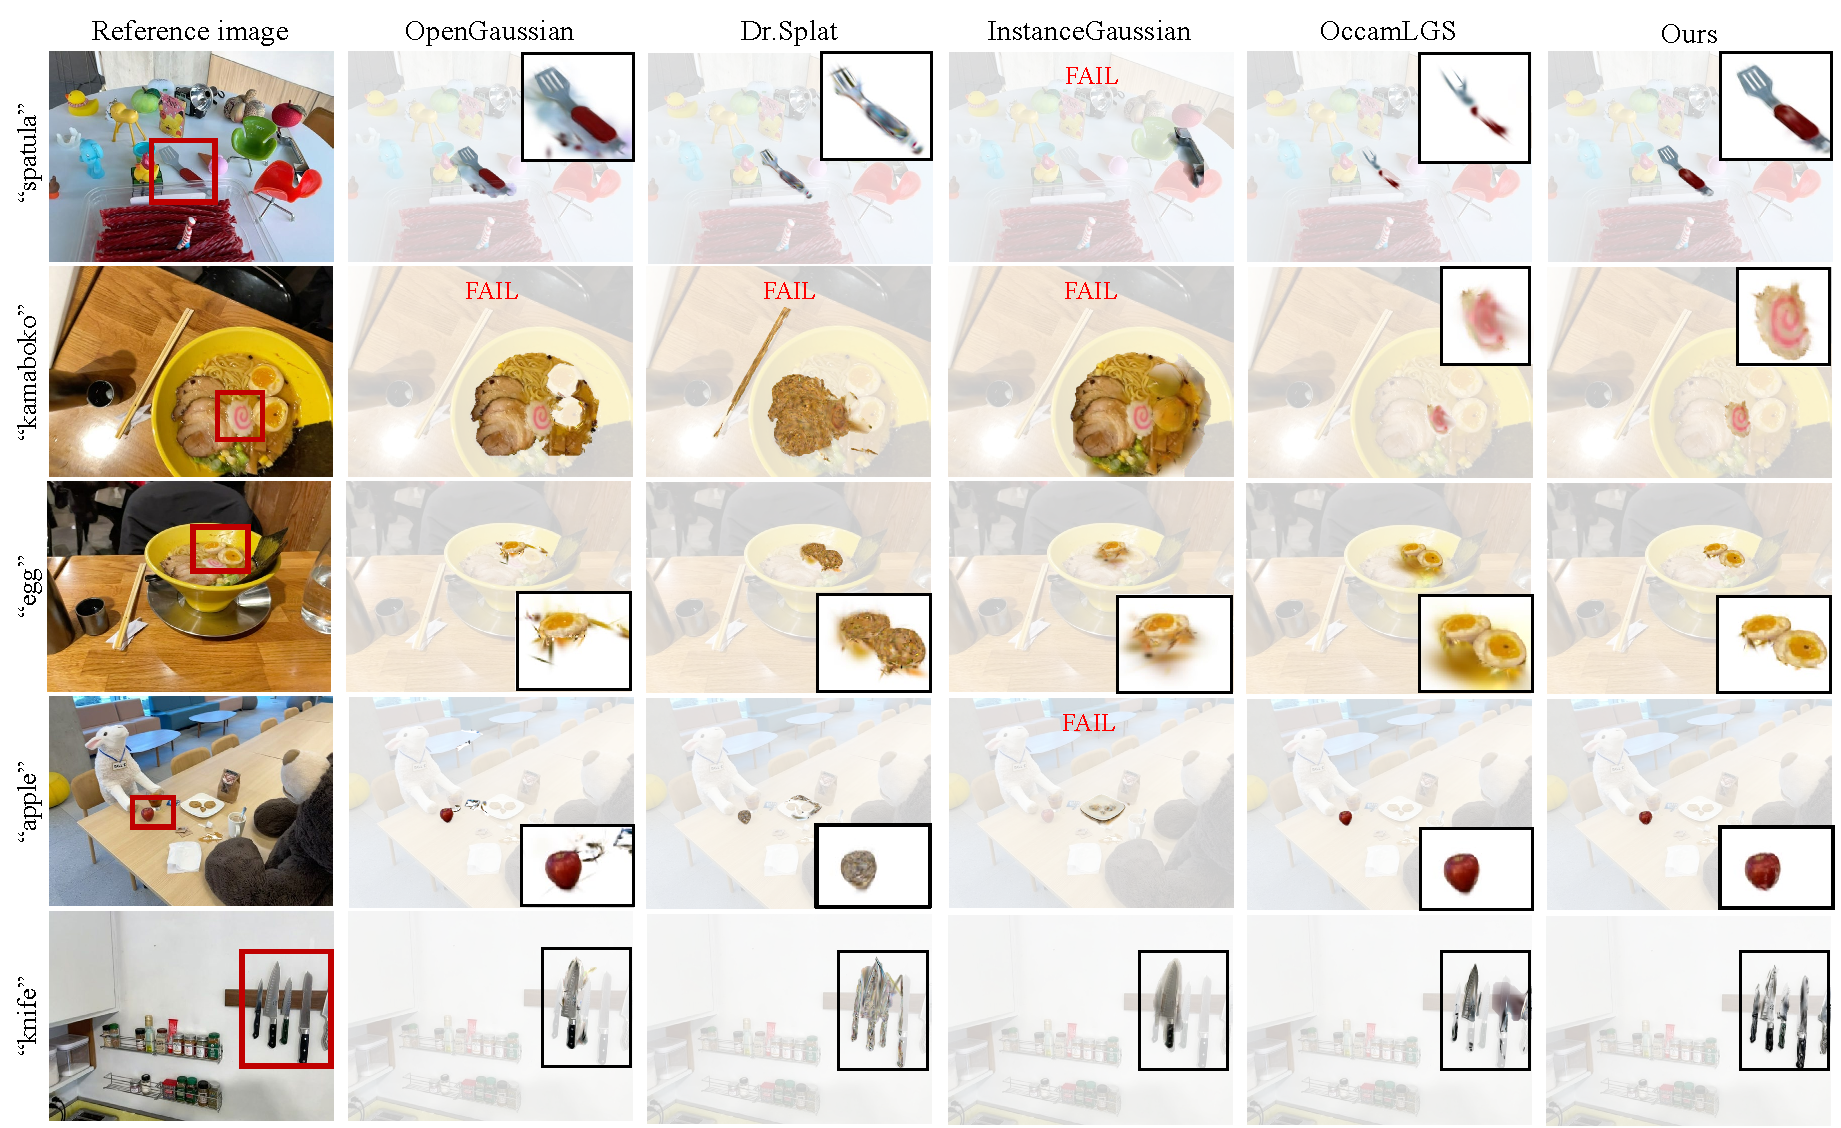
\includegraphics[width=1.\linewidth]{figs/qualitative_lerf_ovs_results.pdf}
\vspace{-5mm}
\caption{Qualitative 3D objects selections on LeRF-OVS~\cite{qin2024langsplat}. We mark as failed those with low or zero IoU with the ground truth (red).}
\label{fig:qualitative_lerfovs}
\vspace{-3mm}
\end{figure*}


\subsection{Analysis on LeRF-OVS dataset}
\tableautorefname~\ref{tab:lerfovs} compares ours with state-of-the-art works on LERF-OVS in 2D and 3D. In 2D, per-view segmentation quality projected from 3D is checked, while in 3D, we directly assess multi-view consistent semantic reconstruction.

\textbf{Quantitatives In 2D.} Our method achieves the highest scores on both mIoU and mAcc, slightly surpassing the mIoU of Occam's LGS~\cite{cheng2024occam} and outperforming LangSplatV2~\cite{li2025langsplatv2}. This improvement is consistent across diverse scenes, particularly in Figurines and Ramen, suggesting that our visibility-aware attribution reduces per-ray semantic noise without sacrificing fine-grained per-view accuracy. While GAGS~\cite{peng2024gags} and LangSplat~\cite{qin2024langsplat} also deliver competitive 2D scores, their performance drops with complex occlusions (\eg, Ramen for GAGS), indicating that their 2D-driven assignments do not fully mitigate cross-view inconsistencies.

\textbf{Quantitatives In 3D.} The advantage of our method becomes more pronounced in 3D, with ours exceeding all baselines by a notable margin. The second best, CAGS~\cite{sun2025cags}, is a substantial 7.2 absolute mIoU points behind. The scene-level analysis reveals that our approach leads in Ramen, Teatime, and Waldo\_Kitchen, and ranks second in Figurines, behind VoteSplat~\cite{jiang2025votesplat} due to its specialized multi-view voting. The gains are especially significant in large, cluttered environments (Teatime, Waldo\_Kitchen), where our contribution-aware aggregation better preserves semantics despite severe occlusions.

The strong 3D consistency of our method contrasts with approaches like LangSplat and LEGaussian~\cite{shi2024language}, whose high 2D accuracy does not translate to 3D performance, likely due to their lack of explicit handling of per-ray contribution and occlusion. Similarly, the post-hoc clustering methods OpenGaussian~\cite{wu2024opengaussian} and SuperGSeg~\cite{liang2024supergseg} exhibit moderate 3D improvements but remain sensitive to upstream semantic drift, thereby limiting their robustness. Our performance relative to Occam's LGS (baseline) is noteworthy: while both adopt streaming updates, our visibility-guided feature attribution yields much better performance in 3D, highlighting the effectiveness of improving the semantic assignment at the feature aggregation stage rather than solely relying on memory-efficient training.

\textbf{Qualitatives in 3D.} 
We show visual 3D results in Figure~\ref{fig:qualitative_lerfovs}. %We evaluate the 3D object selection task on the LeRF-OVS dataset. 
Existing approaches, such as InstanceGaussian~\cite{li2024instancegaussian}, frequently fail by retrieving incorrect objects across multiple scenes. This can be attributed to their reliance on appearance–semantic joint representations, which struggle to distinguish small objects with visually similar appearances. Clustering-based methods struggle with multiple instances that are closely related. For example, querying for \emph{``knife''}, OpenGaussian~\cite{wu2024opengaussian} and InstanceGaussian~\cite{li2024instancegaussian} detect only one out of five knives, whereas Dr.Splat~\cite{drsplat25} and Occam’s LGS~\cite{cheng2024occam} identify all knives but produce indistinct boundaries. In contrast, ours successfully localizes all knives with accurate and sharp delineations. Our approach also demonstrates robustness on challenging small-object queries, such as \emph{``Kamaboko''} and \emph{``egg''} in the \emph{Ramen} scene. These targets lie within a heavily cluttered context (a bowl of ramen), making them particularly difficult to isolate. Competing methods~\cite{wu2024opengaussian, drsplat25, li2024instancegaussian} fail to recognize these objects, while Occam’s LGS correctly retrieves them but with blurred contours. By comparison, ours produces precise boundaries and accurately captures fine object structures. Similar improvements are observed in the \emph{``Spatula''} query, further illustrating that our visibility-aware gating not only mitigates occlusion effects but also enables the recovery of fine-grained details in complex scenes.

\subsection{3D Semantic Segmentation on ScanNet}

\begin{figure*}[t]
\centering
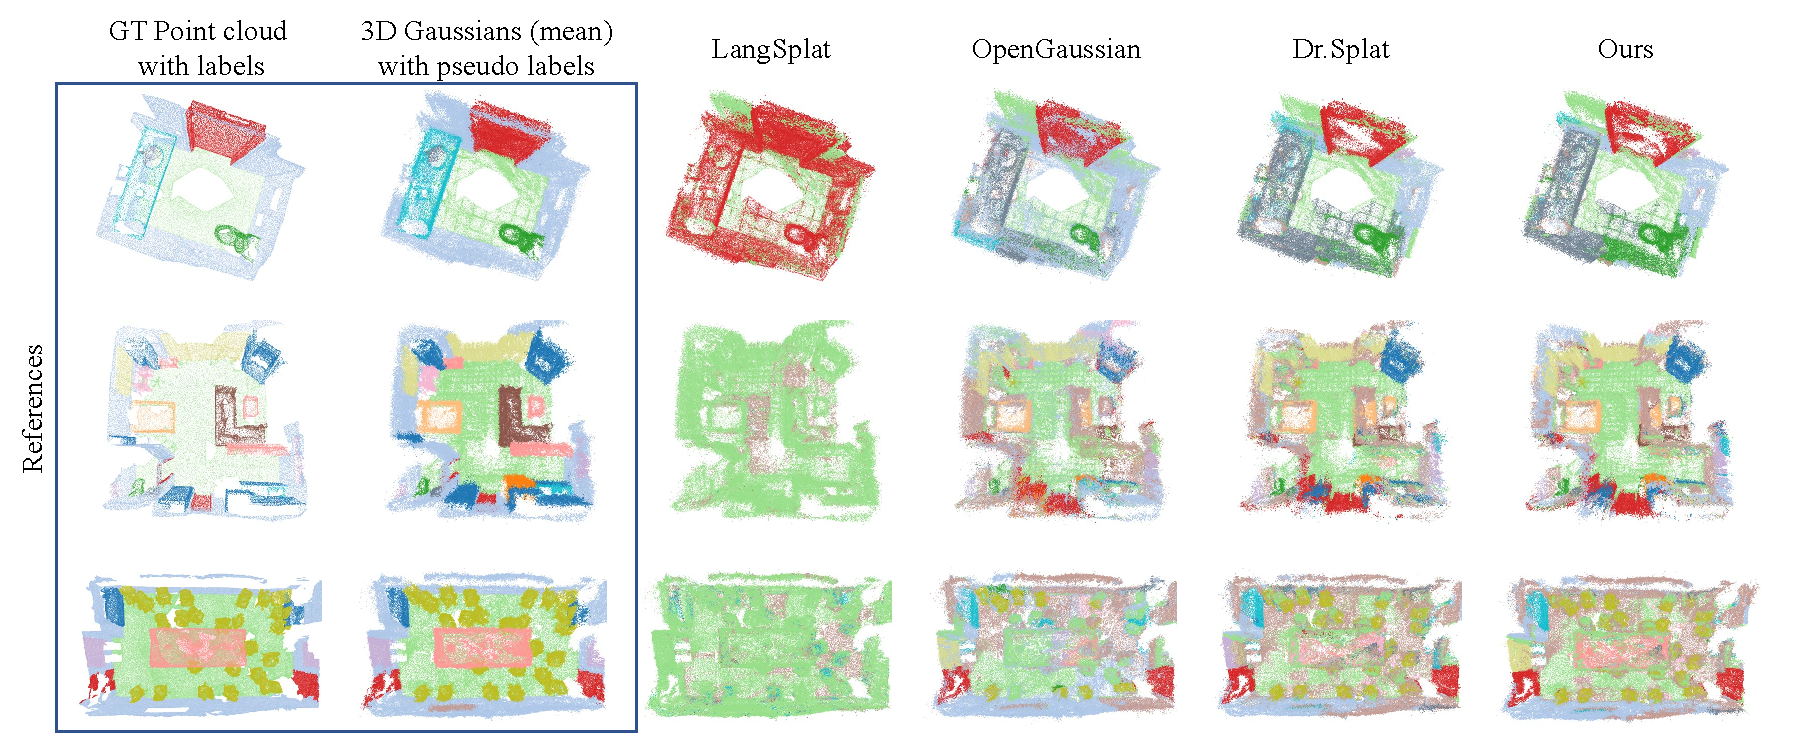
\includegraphics[width=\linewidth]{figs/qualitative_scannet_results.pdf}
\vspace{-9mm}
\caption{Qualitative results of 3D semantic segmentation with 19 classes on the ScanNet-v2 dataset~\cite{dai2017scannet}.}
\label{fig:qualitative_scannet}
~\vspace{-9mm}
\end{figure*}

\begin{table}[t]
\centering
\small
\setlength{\tabcolsep}{2.85pt}
\renewcommand{\arraystretch}{1.1}
\begin{tabular}{lcccccc}
\toprule
& \multicolumn{2}{c}{19 classes} & \multicolumn{2}{c}{15 classes} & \multicolumn{2}{c}{10 classes} \\
\cmidrule(lr){2-3} \cmidrule(lr){4-5} \cmidrule(lr){6-7}
Method & mIoU & mAcc & mIoU & mAcc & mIoU & mAcc \\
\midrule
LangSplat~\cite{kerr2023lerf} & 2.45 & 8.59 & 3.45 & 13.21 & 6.48 & 21.89 \\
OpenGaussian~\cite{wu2024opengaussian} & 27.73 & 42.01 & 29.67 & 46.15 & 39.93 & 57.34 \\
Dr. Splat~\cite{drsplat25} & 29.31 & 47.68 & 33.25 & \nd54.33 & 44.19 & \nd65.19 \\
Occam's LGS~\cite{cheng2024occam} & \nd31.93 & \nd48.93 & \nd34.25 & 53.71 & \nd45.16 & 64.39 \\
\textbf{VALA [ours]} & \fr32.11 & \fr50.05 & \fr35.10 & \fr54.77 & \fr46.21& \fr65.61 \\
\bottomrule
\end{tabular}
\vspace{-2mm}
\caption{Open-vocabulary 3D semantic segmentation task on the ScanNet-v2 dataset~\cite{dai2017scannet} across different amounts of classes.}
\label{tab:openvocab_seg}
\vspace{-5mm}
\end{table}

\textbf{Quantitatives.}  
As reported in Table~\ref{tab:openvocab_seg}, our method achieves the best performance across all evaluation settings, including the most challenging 19-class scenario. Compared to Occam's LGS~\cite{cheng2024occam}, our contribution-aware aggregation is advantageous, demonstrating its ability to handle fine-grained class distributions. While Dr.Splat~\cite{drsplat25} attains competitive accuracy in reduced-category settings, it lags notably in mIoU, indicating weaker spatial consistency. These results confirm that our method achieves robust and precise 3D segmentation across varying label granularities.

% \noindent
\textbf{Qualitatives.}  
Qualitative comparisons are presented in \figureautorefname~\ref{fig:qualitative_scannet}. In the large and complex second room, our method accurately predicts the wall behind the bed (bed in orange), a structure often misclassified by others. In the smaller but more occluded third scene, our method also demonstrates superior 3D segmentation, capturing challenging objects such as the central table more effectively. This ability to recover occluded and fine-scale geometry is particularly beneficial for downstream applications such as 3D object localization. Overall, the qualitative results support the quantitative improvements, highlighting both the robustness and effectiveness of our proposed framework.

\vspace{-1mm}
\begin{table}[b]
  \centering
  \small
  \vspace{-5mm}
  % \setlength{\tabcolsep}{2.1pt}
  \begin{tabular}{lccccc}
    \toprule
    Ref. & Stage A & Stage B & Median & mIoU & mAcc \\
    \cmidrule(lr){1-1} \cmidrule(lr){2-4} \cmidrule(lr){5-6}
    %Occam's LGS~\cite{cheng2024occam} (no gating + weighted mean)  
    O.LGS~\cite{cheng2024occam} & && & 47.22 & 74.86 \\
    % \midrule
    (b) & && cosine & 49.03 & 80.08 \\
    % Occam's LGS + our cosine median  & 49.03 & 80.08 \\
    (c) & \checkmark & & cosine              & 57.24 & 81.25 \\
    (d) &    & \checkmark & cosine  & 55.21 & 80.37 \\
    % first stage B then stage A gating & -- & -- \\
    % Stage A and Stage B gating &57.95&82.55\\
    % \textbf{Full: Stage A + Stage B (ours)}           & -- & -- \\
    \textbf{VALA} & \checkmark & \checkmark & cosine & \textbf{58.02}& \textbf{82.85}\\
    (f) &    \checkmark & \checkmark &  & 52.29 &76.17 \\
    (g) & \checkmark & \checkmark & L1 & 56.03 & 82.42 \\
    % gating + cosine median &  &  \\
    % no gating, with l1 distance    &45.83& 74.75\\
    \bottomrule
  \end{tabular}
  \vspace{-2mm}
  \caption{Ablation on LeRF-OVS. First row is Occam's LGS~\cite{cheng2024occam}, \ie, our baseline. Stages from Section~\ref{sec:gating}, Median from~\ref{sec:median}. All rows share the same data, rasterizer, and hyperparameters.}
  \label{tab:ablation_lerf}
  % \vspace{-5mm}
\end{table}
    
\subsection{Ablation Study}
% \lipsum[1]
We conduct an ablation study on LeRF-OVS~\cite{qin2024langsplat}, averaging the metrics over all scenes. Table~\ref{tab:ablation_lerf} disentangles the contributions of our main components, namely visibility-aware gating and cosine-based geometric median. Starting from the baseline Occam's LGS~\cite{cheng2024occam}, replacing the naive weighted mean with our cosine median (b) already improves performance, highlighting the advantage of robust aggregation in the embedding space. Incorporating visibility-aware gating further boosts results (c-d), where mass-coverage plus threshold gating (c) yields the strongest individual gain, while quantile pruning (d) provides complementary benefits. We also observe that our gating alone (f) is less effective compared to gating along with our robust median (VALA), showing that the precise aggregation is critical to fully exploit visibility cues. Lastly, we compare cosine and L1 (g) as median, with the former delivering superior results. Our full model (VALA) achieves the best overall performance, validating that both visibility-aware gating and cosine-based median aggregation are important for an accurate and view-consistent 2D-3D language lifting.

We refer to the \textbf{Supplementary Material} for additional details and results.